\section{Experiments and Evaluations}
\label{sec:experiments}

We evaluate \ssppp{} against five baselines on three questions: (1)~does
the bounded head reduce predictive accuracy? (2)~does \ssppp{} reproduce
real order-flow structure in closed loop? (3)~which models pass verified
rate calibration? We close with efficiency.

\subsection{Experimental Setup}
\label{sec:setup}
\paragraph{Datasets.}
We benchmark on Coinbase BTC, ETH, and SOL event-driven order flow, seven
days per asset, encoded into $|\mathcal{E}|=62$ atomic types ($20+20+2+20$
over LO/CO/MO/IS, sides, and levels). Validation-split rates are $38.3$,
$47.9$, and $24.0$ events/s: production rates, not subsampled streams.

\paragraph{Baselines.}
All models share the same input embedding and training configuration. They
differ only in the decoder.
\begin{itemize}\setlength\itemsep{1pt}
\item \textbf{LSTM}: a standard LSTM decoder.

\item \textbf{NHP} \citep{Mei2017TheProcess}: the neural Hawkes
  continuous-time LSTM.
\item \textbf{SAHP} \citep{zhang2020self}: an SAHP-style adaptation, not a
  faithful reproduction: a two-layer, four-head causal transformer encoder
  with a softplus intensity held piecewise-constant between events (the
  published decay parameterization is not ported).
\item \textbf{PCT-LSTM} \citep{Shi2022StateSimulation}: the state-dependent
  parallel neural Hawkes process (CT4LSTM-PPP) \emph{without its exogenous
  market-state input}, which the closed-loop protocol cannot supply (this
  may cost it accuracy); the event-driven cell is ported unchanged.
\item \textbf{\sppp{}} \citep{chang2025ctssm}: our factorized, uncapped
  benchmark implementation: identical backbone to \ssppp{}, scalar softplus
  rate with no ceiling (Background; the published head is per-type).
\end{itemize}

\paragraph{Training and evaluation protocol.}
Each model trains per asset with sequence length 1024, non-overlapping
windows, identical gradient-step counts, and three training seeds. The fixed
1024-event context spans only ${\sim}20$--$40$\,s of market time at these
rates, so long-memory structure leans entirely on carried state. Evaluation is
strict end-to-end:
\begin{itemize}\setlength\itemsep{1pt}
\item \textbf{Prediction} is scored on \emph{every} genuine test event by a
  lossless streaming evaluator with carried state (one cold start per genuine
  segment boundary); it hard-fails if any event goes unscored. NLL uses a
  32-point log-spaced quadrature per gap; type accuracy is conditional on
  the observed next-event time; MAE is expected-time absolute error on a
  60\,s horizon (definitions in the appendix).
\item \textbf{Simulation} uses carried-state closed-loop roll-outs
  ($32\times600$\,s, three roll-out seeds per checkpoint) against
  equal-duration bootstrap samples of real segments. \ssppp{} samples by
  Ogata thinning with its exact closed-form ceiling; the baseline heads
  expose no closed-form dominating rate and share a common
  compensator-inversion sampler. Stylized facts are computed on an
  order-flow proxy (signed counts of price-moving events per 1\,s bucket),
  identically for real and simulated streams (appendix).
\item \textbf{Calibration}: models are rate-calibrated before scoring by a
  one-dimensional bisection on the time-rescaling constant $\kappa$,
  targeting the \emph{validation}-split rate; a full-scale validation
  roll-out must then reproduce the target within 15\% (protocol in the
  appendix). Failing checkpoints are excluded and the failure is reported as
  a result. SAHP is the exception: after its free-running rate collapsed on
  every asset, calibration was not attempted for it (protocol decision) and
  it is reported uncalibrated (\dag).
\item \textbf{Statistics}: roll-out seeds are averaged within each checkpoint.
  95\% CIs are $t$-based across three training seeds, indicative only at
  this sample size. Any batch failure or non-finite value aborts the run.
  Released scripts regenerate every table and figure.
\end{itemize}



\begin{table*}[t]
\centering\footnotesize
\setlength{\tabcolsep}{2.3pt}
\begin{tabular}{lcccccc}
\toprule
 & \multicolumn{2}{c}{BTC} & \multicolumn{2}{c}{ETH} & \multicolumn{2}{c}{SOL}\\
\cmidrule(lr){2-3}\cmidrule(lr){4-5}\cmidrule(lr){6-7}
model & overall$\downarrow$ & ACC$\uparrow$ & overall$\downarrow$ & ACC$\uparrow$ & overall$\downarrow$ & ACC$\uparrow$\\
\midrule
\nhp{} & \textbf{-1.07$\pm$0.01} & \textbf{0.449$\pm$0.003} & -0.81$\pm$0.03 & 0.341$\pm$0.006 & 0.53$\pm$0.01 & 0.184$\pm$0.004\\
LSTM & -0.44$\pm$0.40 & 0.411$\pm$0.015 & 0.15$\pm$0.04 & 0.288$\pm$0.003 & 1.34$\pm$0.25 & 0.141$\pm$0.005\\
SAHP\,\dag & -0.93$\pm$0.01 & 0.412$\pm$0.001 & -0.60$\pm$0.01 & 0.297$\pm$0.004 & 0.67$\pm$0.02 & 0.155$\pm$0.003\\
PCT-LSTM & -0.60$\pm$0.08 & 0.313$\pm$0.010 & -0.34$\pm$0.10 & 0.248$\pm$0.007 & 0.89$\pm$0.03 & 0.105$\pm$0.004\\
\sppp{} & -0.39$\pm$0.25 & 0.439$\pm$0.002 & -0.38$\pm$0.22 & 0.331$\pm$0.008 & 0.67$\pm$0.49 & 0.182$\pm$0.002\\
\ssppp{} & -0.87$\pm$0.12 & 0.448$\pm$0.001 & \textbf{-0.87$\pm$0.08} & \textbf{0.345$\pm$0.003} & \textbf{0.27$\pm$0.05} & \textbf{0.192$\pm$0.001}\\
\bottomrule
\end{tabular}
\caption{Prediction per genuine test event (mean $\pm$ 95\% CI over three
training seeds; streaming lossless evaluator). NLL = overall negative
log-likelihood (time $+$ mark); ACC = next-type accuracy at the observed
event time; MAE = expected-time mean absolute error in seconds (60\,s
evaluation horizon). \ssppp{} wins NLL and ACC on ETH and SOL and
ties \nhp{} on BTC accuracy; \spppu's MAE column reflects expected times
that run into the evaluator's horizon clamp on a subset of states.}
\label{tab:multiasset}
\end{table*}

\subsection{Prediction Quality}
\label{sec:prediction}
\ssppp{} leads NLL and type accuracy on two of the three assets, and
bounding the intensity did not reduce predictive performance in these
experiments. In Table~\ref{tab:multiasset}, \ssppp{} wins overall NLL on
SOL by a wide margin ($0.27$ vs.\ the strongest baseline's $0.38$) with the
best accuracy ($0.192$ vs.\ $0.184$), wins both outright on ETH ($-0.87$
vs.\ PCT-LSTM's $-0.84$; $0.345$ vs.\ \nhp's $0.341$), and on BTC ties
\nhp{} on marks ($0.448$ vs.\ $0.449$) while conceding overall likelihood.
Expected-time MAE is within $0.030$--$0.050$\,s of the truth on every
asset, approximately 1--3\,ms behind the best model per asset (PCT-LSTM has
the lowest MAE on ETH and SOL); the uncapped \spppu{} is pathological
($2.3$, $10.2$, $46.2$\,s), consistent with near-zero-intensity states
whose expected-time integral runs to the evaluation horizon.
% The remaining gap to \nhp{} is in timing on BTC, and a per-gap decomposition
% of timeNLL $= -\log\lambda(t_i) + \Delta u_i$ (event term $+$ compensator
% mass) shows it is not about bursts: the state-space family's event terms beat
% \nhp's ($-4.87$ \ssppp{} vs.\ $-4.29$). The entire gap is compensator mass
% in \emph{quiet gaps}: mean per-gap rescaled mass is $1.85$ (\ssppp) and
% $2.38$ (\sppp) against \nhp's near-ideal $1.07$ (target $1$), with the
% excess accruing in gaps beyond $0.1$\,s: \ssppp{} integrates $4.3$ units
% of intensity across a $0.5$--$2$\,s lull where \nhp{} integrates $0.8$. The
% insight is mechanistic: \nhp{} decays toward a \emph{learned steady state}
% that tracks the falling empirical hazard of long gaps, while the state-space
% family, with no dedicated resting-rate parameter, stays hot through lulls.
% This quiet-gap cost is the deliberate price of stability; what it buys is the
% subject of the next two subsections.




\begin{figure*}[t]
\centering
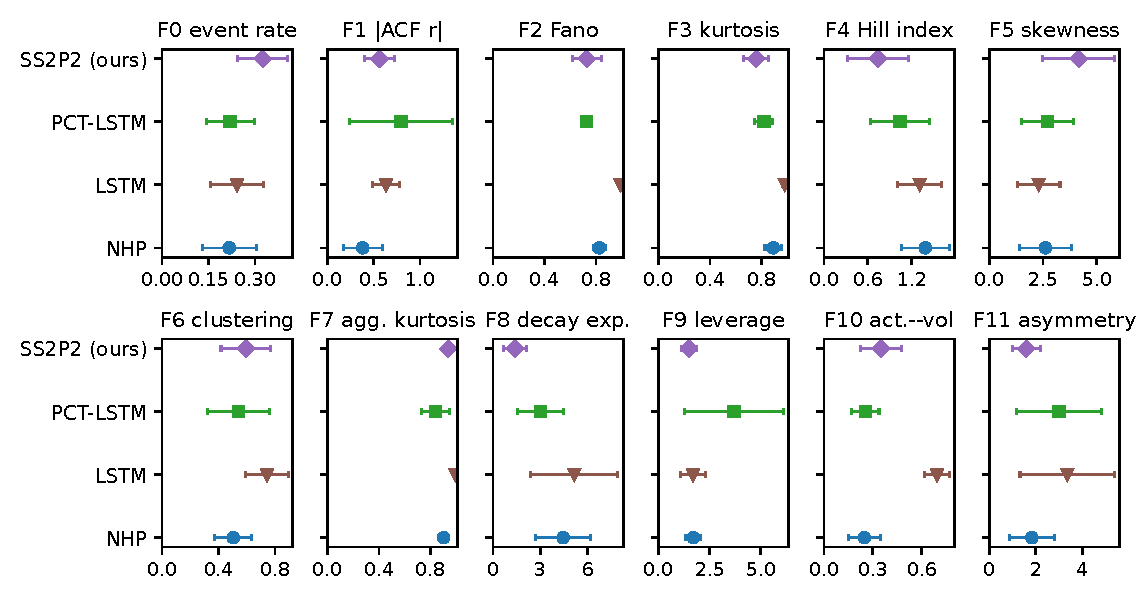
\includegraphics[width=0.75\textwidth]{figs/fig_forest}
\caption{The stylized-fact battery on the order-flow proxy (identical
construction for real and simulated streams), pooled across assets:
relative error vs.\ real for facts F0--F11 (whiskers = 95\% $t$-CI over
asset--checkpoint pairs, indicative at $n{=}3$ seeds; roll-out seeds
averaged within checkpoint). \spppu{} and SAHP omitted: too few calibrated
checkpoints.}
\label{fig:forest}
\end{figure*}

\subsection{Simulation Quality}
\label{sec:simulation}
\ssppp{} is the only model pairing reliable closed-loop simulation with
top-tier prediction; the two strongest baseline predictors are unusable or
erratic in closed loop. SAHP's free-running rate collapses to
$5$--$16$\,ev/s against matched real segments at $20$--$35$\,ev/s, under
half the real rate on every asset; per protocol it was not calibrated
(\dag{} in Table~\ref{tab:multiasset}). The uncapped \spppu{} drifts hot
instead: 6 of 9 checkpoints, all three on SOL among them, fail verified
calibration (Table~\ref{tab:caloutcomes}), and the three that pass are
erratic, with roll-out Fano relative errors of $0.27$, $2.2$, and $6.0$:
simulated dispersion quality is seed luck.

Among the remaining models, Figure~\ref{fig:forest} scores the roll-outs on
the stylized-fact battery (twelve facts on the order-flow proxy), pooled
across assets. \ssppp{} has the lowest mean relative error on five of
twelve (heavy tails F3, Hill index F4, volatility decay F8, leverage F9,
asymmetry F11), ties PCT-LSTM for best on the Fano panel F2 ($0.73$ both),
and is mid-pack on the rest; confidence intervals overlap heavily on most
panels, so we read the figure as broad competitiveness, not dominance. The F2 panel still separates
the families most sharply: the LSTM pins at ${\approx}0.99$ with a
negligible interval because it simulates a near-Poisson stream, the
trivially-stable end of the trade-off, while real Fano rises from
${\sim}40$--$70$ at 1\,s to ${\sim}340$--$1400$ at 50\,s across assets.
\nhp, the best BTC predictor, leads the rate and activity panels (F0, F10)
but is mid-pack on burst structure; PCT-LSTM matches \ssppp{} on F2 and
leads aggregated kurtosis F7, but has the weakest type accuracy in
Table~\ref{tab:multiasset}. Prediction and simulation quality are distinct
axes: no baseline wins both, and only the bounded design tracks burst
structure while predicting at the top of the table.

\subsection{Calibratability}
\label{sec:calibratability}
Post-hoc rate calibration applies to \emph{every} decoder, because a
constant $\kappa$ rescales sim-time intensity while preserving conditional
type ratios at a fixed history; we calibrate every model except SAHP
(excluded above) and treat the \emph{outcome} as a result. The
protocol is falsifiable: probes must bracket and converge to the validation
target, a full-scale roll-out must reproduce it within 15\%, and every
failure is reproducible (deterministic probe seeds; retried failures
reproduce their brackets bit-identically).

\begin{table}[t]
\centering\small
\setlength{\tabcolsep}{6pt}
\begin{tabular}{lcccc}
\toprule
 & Gemini ETH & CB BTC & CB ETH & CB SOL\\
model & $\sim$4\,ev/s & 38\,ev/s & 48\,ev/s & 24\,ev/s\\
\midrule
\nhp{} & 3/3 & 3/3 & 3/3 & 3/3\\
LSTM & 3/3 & 3/3 & 3/3 & 3/3\\
SAHP\,\dag & \multicolumn{4}{c}{\emph{model-level divergence: reported uncalibrated}}\\
PCT-LSTM & 3/3 & 3/3 & 3/3 & 3/3\\
\sppp{} & \textbf{2/3} & \textbf{1/3} & \textbf{1/3} & \textbf{0/3}\\
\ssppp{} & 3/3 & \textbf{2/3} & 3/3 & 3/3\\
\bottomrule
\end{tabular}
\caption{Checkpoints passing calibration $+$ full-scale verification, out of
three training seeds per asset (bold marks failures). The uncapped \spppu{}
head fails on 6 of 9 checkpoints, including \emph{all three} on SOL where no
usable simulator remains, while the bounded \ssppp{} head verifies on all
nine. SAHP's free-running rate collapses on every asset; it was not
calibrated (protocol decision) and is reported uncalibrated.}
\label{tab:caloutcomes}
\end{table}

Whether a checkpoint passes this test is measurable, and in our benchmark
the bound decided it: Table~\ref{tab:caloutcomes} shows the bounded
\ssppp{} head verifying on \emph{all nine} checkpoints, while the uncapped
\spppu{} head fails on 6 of 9, and on SOL the model class is excluded
outright.

Figure~\ref{fig:ladder} shows the failure in detail (shaded band: the
bisection's $\pm5\%$ probe tolerance; the 15\% rule applies to full-scale
verification). The failing BTC \spppu{} checkpoint responds extremely
sharply to $\kappa$: an $8\times10^{-4}$ change moves the probe rate across
the band ($34.8\to42.3$\,ev/s, target $38.3$), repeat probes at fixed
$\kappa$ differ by tens of percent (nearly $2\times$ in places), and
full-scale verification then missed by 22\%. This rescaling sensitivity is
consistent with near-critical behavior; the procedure found no multiplier
satisfying verification, while the \ssppp{} response crossed the same
target smoothly on every asset. The same uncapped head whose
near-zero-intensity states produce \spppu's pathological expected-time
tail (Table~\ref{tab:multiasset}) also produced the erratic closed-loop
response; both problems were absent under the softmin bound in every
reported run --- an empirical regularity, not a theorem.

\begin{figure}[t]
\centering
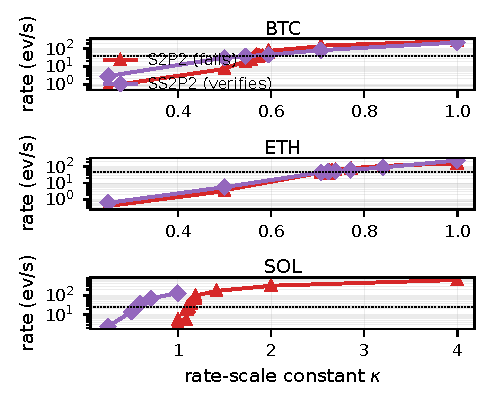
\includegraphics[width=0.77\columnwidth]{figs/fig_cal_ladder}
\caption{Failing \spppu{} checkpoints respond near-discontinuously to the
rescaling constant $\kappa$ on every asset, most extremely on SOL; verified
\ssppp{} checkpoints cross each target smoothly. Probe ladders, seed-1
checkpoints; shaded band = $\pm5\%$ probe tolerance around the validation
target.}
\label{fig:ladder}
\end{figure}

\subsection{Efficiency Analysis}
\label{sec:efficiency}
The backbone is also computationally advantageous once its per-event
sequential loop is replaced by a Hillis--Steele prefix scan
\citep{hillis1986scan} over the ZOH recurrence (equivalent up to
floating-point order; maximum observed state/gradient discrepancy
$2\!\times\!10^{-4}$). On one GPU (Table~\ref{tab:speed}, appendix; ETH
checkpoints) the scan collapses the \sppp-family training step from
$3.5$\,s to ${\sim}0.06$\,s: attention-class speed, $60\times$ over the
loop, $73\times$ over the CT-LSTM. For sampling, \ssppp's exact ceiling makes Ogata
thinning available with a \emph{constant} dominating rate (mean acceptance
$0.54$ on ETH, ${\sim}1.9$ proposals per event): exactness costs
${\sim}2.5\times$ against the shared inversion sampler, and both run far
above real time ($353$ vs.\ $48$ events/s on the fastest asset).
% AUTHOR ACTION REQUIRED: archive the speed-bench raw logs (train-step and
% thinning acceptance) with the release; confirm the PCT-LSTM row was
% re-measured with the current SD-PNHP backbone.
